\label{fs-acker-design}

\begin{figure}[htbp]
  \centering
  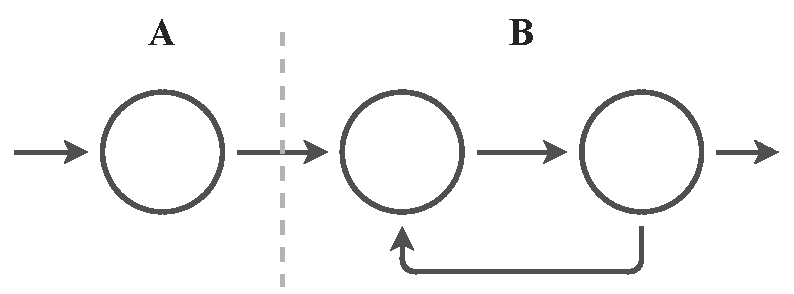
\includegraphics[width=0.5\textwidth]{pics/graph-segments.pdf}
  \caption{Graph segmentation}
  \label{graph-segments}
\end{figure}

\ref{graph-segments}

In this section, we focus on the core concepts of our dependency tracking method. Within the design of this mechanism, we aim at providing the following properties:
\begin{itemize}
    \item Fine granularity of tracking: for each input element (or for each small group of input records), it should be possible to determine when the element has been entirely processed independently from other items.
    \item Operator-level or block-level locality of tracking: the mechanism should provide independent notifications for various blocks of a dataflow.
    \item Notifications order preservation: the order of notifications should not contradict the order of input elements arrival with respect to wall time.
    \item Cyclic dataflows support: our tracking technique should be suitable for cyclic dataflow graphs. This feature substantially extends the applicability of a dependency tracking method.
\end{itemize}

Our dependency tracking mechanism is inspired by Apache Storm \acker\ technique that we mentioned in the previous section. Firstly, each input data item is assigned with a unique label and a 64-bit random number. When an operator transforms elements, it preserves the label but assigns a new random number to the transformed record. All operators send tuples $(label, number)$ on each input and output element to a special agent called \acker . \acker\ XORs all random numbers grouped by the labels. 

Note that each random number is sent to \acker\ precisely two times: when an operator sends a new transformed element downstream and when the next operator receives it. Therefore, if the XOR checksum for some label becomes zero, it means that all elements with that label are successfully processed. \acker\ broadcasts notifications on these events.

To avoid checksum becoming zero until all elements with a specified label are entirely processed, operators firstly send tuples $(label, number)$ for output elements and only after that for the input. There is a small probability that the random numbers will be XORed into zero accidentally, but it can be neglected in practice~\cite{apache:storm:acker}.

We can illustrate \acker\ as a table with two columns: label and checksum. Table~\ref{ack_table} illustrates such table. According to this example, elements with label $b$ have been entirely processed, while records with labels $a$ and $c$ are still in processing.

\begin{table*}
  \begin{minipage}[b]{.40\textwidth}
    \centering
    \caption{Acker table}
    \begin{tabular}{|c|>{\bfseries}c|c|c|} 
      \hline
      Released & Label & XOR & Global Time  \\ \hline \hline
      \checkmark & a & 000 & 1 \\ \hline
      & b & 101 & 4 \\ \hline
      \checkmark & c & 000 & 3 \\ \hline
      & d & 110 & 2 \\ \hline
    \end{tabular}
  \end{minipage}\qquad
  \begin{minipage}[b]{.40\textwidth}
    \centering
    \caption{Acker + ordering}
    \begin{tabular}{|c|>{\bfseries}c|c|c|} 
      \hline
      Released & Global Time & XOR  \\ \hline \hline
      \checkmark & 1 & 000 \\ \hline
      & 2 & 110 \\ \hline
      blocked by 2 & 3 & 000 \\ \hline
      & 4 & 101 \\ \hline
    \end{tabular}
  \end{minipage}
  \begin{minipage}[b]{.40\textwidth}
    \centering
    \caption{trAcker}
    \begin{tabular}{|c|>{\bfseries}c|c|c|c|} 
      \hline
      Released & Global Time & Segment & Local XOR & XOR  \\ \hline \hline
      \multirow{2}{*}{\checkmark} & \multirow{2}{*}{1} & A & 000 & \multirow{2}{*}{000} \\ \cline{3-4}
      & & B & 000 & \\ \hline
      \multirow{2}{*}{} & \multirow{2}{*}{2} & A & 000 & \multirow{2}{*}{110} \\ \cline{3-4}
      & & B & 110 & \\ \hline
      \multirow{2}{*}{} & \multirow{2}{*}{3} & A & 000 & \multirow{2}{*}{000} \\ \cline{3-4}
      & & B & 000 & \\ \hline
      \multirow{2}{*}{} & \multirow{2}{*}{4} & A & 100 & \multirow{2}{*}{101} \\ \cline{3-4}
      & & B & 001 & \\ \hline
    \end{tabular}
  \end{minipage}
  \label{ack_table}
\end{table*}

\acker\ mechanism provides for the fine granularity of tracking and cyclic dataflows support out-of-the-box. However, only the uniqueness property of labels does not allow \acker\ to support block-level locality and notifications order preservation. Further, in this section, we design a more sophisticated structure of labels. Using these extended labels, we propose a \tracker\ mechanism that complements \acker\ and provides for all desired dependency tracking properties. 

\subsection{\tracker\ mechanism}

\subsection{Ordered labelling}

%todo: посчитать вероятности того, что акер обнулится

% Then, each operator shares information about labels of all arriving and outgoing elements with an agent called {\em \tracker}.

% Our dependency tracking mechanism bases on the following scheme. Firstly, each data item is assigned with a special label. Then, each operator shares information about labels of all arriving and outgoing elements with a (potentially distributed) agent called {\em \tracker}. Thus, \tracker\ monitors all in-flight data items within a system. Finally, \tracker\ provides notifications when it ensures that elements with specific labels have been entirely processed.

% In section~\ref{labeling}, we introduce a concept of {\em global time}: the ordered labels that are assigned to data items. This framework allows us to logically group an input stream into small ordered pieces and to monitor the descendants of these pieces independently. We describe the method of global time generation and the ordering properties that it provides.

% In section~\ref{tracker_mechanism}, we propose the tracking mechanism itself and formulate basic requirements that a stream processing system must satisfy in order to employ \tracker . We demonstrate the way \tracker\ aggregates service information from operators, and how it uses the concept of global time to guarantee the order of notifications and fine granularity of tracking. We discuss a technique that allows \tracker\ to provide for the block-level locality. 

% Finally, in Section~\ref{tracker_examples}, we illustrate our tracking mechanism within two practical problems: completeness monitoring and state snapshotting.

% \subsection{Data items labeling} \label{labeling}

% \subsubsection{Global time concept} \label{fs-acker-gt}

% In Storm \acker\ completeness monitoring mechanism, which is a source of inspiration for our method, all input elements are assigned with a random number. \acker\ notifies the system when an element with some specific number has been entirely processed. If \acker\ is not producing notifications for some elements for quite a long time, it may indicate the loss of the elements. In such setting, the order of notifications does not matter because they may only cause reprocessing of certain elements that is enough for {\em at-least-once} delivery guarantee~\cite{Toshniwal:2014:STO:2588555.2595641}.

% On the other hand, a consistent state snapshotting problem requires more strict ordering properties. To provide for {\em exactly-once} guarantee, the system should periodically save the state of all operators only after a notification that some set of input elements have been already proceseed~\cite{thepaper}. These notifications should be conformed with the order of input items arrival. If the notification that the input element arrived at (wall) time $\tau$ has been entirely processed is generated after the same notification for input element arrived at time $\tau + 1$, state snapshots may become inconsistent~\cite{2015arXiv150608603C}.

% In the marker-based approach that is commonly used for state snapshotting problem~\cite{Carbone:2017:SMA:3137765.3137777}, ordering properties are naturally provided by the implementation itself. As we mentioned in Section~\ref{existing_solutions}, markers are injected as ordinary elements and cannot be reordered with them. Hence, notifications are always provided in the order that is consistent with the ingestion of input items.

% The core concept that allows our method to preserve the order of notifications is \textit{global time}. Global time is a special label that a stream processing system assigns to each input element. As we mentioned above, our dependency tracking mechanism monitors global times of in-flight records within a system. Hence, our mechanism can provide notifications with respect to the order of global times. If global time ordering is conformed with the order of input elements arrival, it will ensure the notifications order preservation.

% %требования к меткам
% %timing - wall time, упорядоченность, system time
% %global time = approximation wall time
% %если 1 - все ок wall time, если распределенно, то приближенно
% %global time, не обязательно уникальный даже на одной машине
% %лемма доказывает, что с аппроксимацией все ок
% %пояснить, что если global time не уникальный, то за них нотификация приходит одна
% %group commit
% %VLDB 2017, time oracle, но нам не так важно и тогда еще более fine-grained

% The global time order is based on the assumption that we are able to order input elements up to some difference in wall time. In a case where all elements are coming to the system through the same node, this assumption is natural since the role of global time can be played by a system time of element ingestion. On the other hand, if elements are coming from different nodes, we can compare generation times up to some guaranteed maximum system time difference $\delta$. 

% This way, we can split the whole input stream into pieces of time with length $\delta$ that are comparable by this mechanism. We call the time associated with each piece \textit{global time} $t$. Hence, if input elements are arriving through the single node, all elements will be assigned with different global times. Otherwise, some elements can have the same global time. The number of elements that bear the same global times determines the granularity of tracking and depends on the input items rate and the maximum system time difference between nodes $\delta$. In practice, it is possible to synchronize system times between nodes up to 10 milliseconds difference~\ref{forgot} that can ensure fine granularity of tracking.

% Lemma~\ref{gt-lemma} allows us to connect wall time with the \textit{global time} in a regular way. It states that all elements before true (wall) time $\tau$ are processed if all elements of \textit{global time} $\tau - \delta \le t \le \tau + \delta$ are processed. Therefore, if a tracking mechanism provides notifications in the order of global times, it will be suitable for the state snapshotting problem.

% \begin{lemma}
% \label{gt-lemma}
% If all elements of \textit{global time} less or equal to $t + 1$ are processed, then all elements of wall time $\tau < t$ are processed.
% \end{lemma}
% \begin{proof}
% Element of wall time $\tau$ can be assigned to three different global times due to lack of system time synchronization:
% \begin{itemize}
%     \item input node that has time later then the wall time, in the worst case this time is $\tau - \delta$ that belongs to global time $t - 1 \le t + 1$;
%     \item node that has precise time $\tau$ that belongs to global time $t \le t + 1$;
%     \item and in the worst case the element comes to front with time greater then actual $\tau + \delta$ this time belongs to $t + 1 \le t + 1$ global time.
% \end{itemize}
% as one can see all these cases give the global times less or equal than $t + 1$ which is supposed to be processed.
% \end{proof}

% % This connection is crucial when single client connects to different input nodes of the system (e.g. round-robin balancing). The same semantic is used in markers~\cite{Carbone:2017:SMA:3137765.3137777} concept: instead of global times conditions they simultaneously send a special item from all input nodes and after these elements reach the end of the pipeline generate the outputs of the current piece of input.

% \subsubsection{Glabal time transformation}

% In previous section we used a notion of processed elements. By elements processing we mean the chain of operations induced by some input elements. This chain is defined by logical execution graph of operations. Each node in this graph is a user-defined operation that process input elements one by one and outputs elements, that are then routed according to output node edges to some other operations. We suppose that output elements $O$ of each operation $f$ has the global time of its elements not lower than the global time of the input element $i$.

% \begin{equation}
%     O = f(i), \forall o \in O: t(o) \ge t(i)
% \end{equation}

% The dependencies rule could be even more strict, if we don't allow cycles in execution graph: the output global time will be exactly the global time of the input element. Though, in case of back-links, we want to be able to delay element to influence the future elements and this limits us to the proposed conditions. In this case we regard such elements as postponed input and remove them from consideration at time $t(i)$. As an example of such back-links we can use Nayad cycle counters mechanism~\cite{Murray:2013:NTD:2517349.2522738}. In their scheme they allow to delay element persistence in the system for more than one generation.

% Using this assumption on the global time dependencies, we can easily proof that if system contains no elements of global time $t < t_0$, then no elements of time $t$ will be generated in future.

% \subsection{\tracker\ 's mechanism} \label{tracker_mechanism}
% In previous sections we have defined the main assumptions needed for \tracker\ to function. Using this assumptions we are now ready to define the tracking mechanism itself. We follow the idea of Acker introduced in Storm~\cite{Toshniwal:2014:STO:2588555.2595641}. The original idea is to send random long markers on each item before network transfer and after it. This way we are able to ensure that no elements are ``hang'' in the network using a single XOR operation on the set of such markers. We use this idea a bit differently: we track the way of the element down to output sending random markers in the following situations:
% \begin{itemize}
%     \item element enters the system;
%     \item element is generated by operation;
%     \item element is processed by some operation;
%     \item element is ready for output.
% \end{itemize}
% Following these rules the accumulator element becomes zero iff all descendants of the input element are ready for the output. The next step is to group tracking of the elements by their global time. If such accumulator becomes zero, this means that all elements of this global time are successfully processed. To accumulate markers system-wide we introduce \tracker\ agent which is responsible for gathering tracking information and notification of interested agents on complete processing of the elements of the same global time. The implementation details of the \tracker\ are discussed in Section~\ref{fs-acker-impl}.

% Using introduced mechanism we are now able to define the rule for defined in Section~\ref{fs-acker-gt} semantic. If all accumulators for global time $t \le t_0 + 1$ are empty, we can release the output elements induced by input of time $t_0$ to preserve the wall time order of the input elements. The proof of this statement directly follows our assumptions and \tracker\ guarantees.

% Notably, if execution graph has no cycles and global time equals the global time of the input element, the condition on all accumulators $t \le t_0 + 1$ could be relaxed to $t = \{t_0, t_0 + 1\}$ which allows to make implementation of the \tracker\ even more straightforward.

% \subsection{Examples} \label{tracker_examples}
% In this section we show the application of the introduced mechanism to two popular tasks emerging in stream processing: completeness monitoring and state snapshotting. These tasks are usually addressed by different algorithms by \tracker\ allows to solve them both with introduction of a single agent.
% \subsubsection{Completeness monitoring}

% \subsubsection{State snapshotting}
